\chapter{Stato dell'arte}
\label{chap:stateofart}
In questo capitolo si illustreranno le principali tecnologie adottate, spiegandone il funzionamento e le motivazioni che hanno portato alla loro scelte, preferendole alle alternative.

\section{Programmazione Object-Oriented}
La Programmazione ad Oggetti rappresenta, senza dubbio, il modello di programmazione più diffuso ed utilizzato degli ultimi dieci anni.
Le vecchie metodologie come la programmazione strutturata e procedurale, in auge negli anni settanta e punto di riferimento per lo sviluppo software, sono state lentamente ma inesorabilmente superate a causa degli innumerevoli vantaggi che sono derivati dall’utilizzo del nuovo paradigma di sviluppo. Via via che gli orizzonti della programmazione diventavano sempre più ampi, si andavano evidenziando i limiti delle vecchie metodologie. In particolare, un programma procedurale mal si prestava a realizzare il concetto di \texttt{componente software}, ovvero di un prodotto in grado di garantire le caratteristiche di \textit{riusabilità}, \textit{modificabilità} e \textit{manutenibilità}.
\subsection{Le origini}
Per comprendere meglio il significato di \textsl{programmare per oggetti} è necessario comprendere cosa significhi non farlo. In questa sezione si procederà con una breve analisi dei precursori dell'\textit{Object Oriented Programming}.

\subsubsection{Programmazione non strutturata}
 In questo paradigma il programma è costituito da \textit{un unico blocco di codice detto “main”} dentro il quale vengono manipolati i dati in maniera totalmente sequenziale. Qui i dati sono rappresentati soltanto da variabili di tipo globale, ovvero visibili da ogni parte del programma ed allocate in memoria per tutto il tempo che il programma stesso rimane in esecuzione. È facile intuire come ciò comporti un notevole svantaggio. Questo tipo di programmazione comporta ridondanza nel codice e un'enorme spreco di risorse del sistema.
\begin{figure}[H]
    \centering
    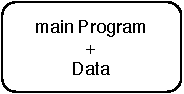
\includegraphics[width=0.20\textwidth]{images/01_1_non_structured_data.pdf}
    \caption{Programmazione non strutturata}
    \label{fig:nonstructured-programming}
\end{figure}

\subsubsection{Programmazione procedurale}
Il concetto base di questo tipo di programmazione è quello di raggruppare i pezzi di programma ripetuti in porzioni di codice utilizzabili e richiamabili ogni volta che se ne presenti l’esigenza. Le porzioni di codice con queste caratteristiche prendono il nome di \textit{procedure}. Ogni procedura può essere vista come un \textit{sottoprogramma che svolge una ben determinata funzione} e che è visibile e richiamabile dal resto del codice. La programmazione procedurale rappresenta un notevole passo in avanti rispetto a quella non strutturata, in quanto ne supera i limiti di ridondanza e garantisce una migliore gestione della memoria di sistema. Il vantaggio di una procedure sta nell'utilizzo dei parametri, allocati in memoria solo nel momento in cui una quest'ultima viene chiamata. Il \textit{main continua ad esistere} ma al suo interno presenta esclusivamente le invocazioni alle procedure definite dal programma. 
\begin{figure}[H]
    \centering
    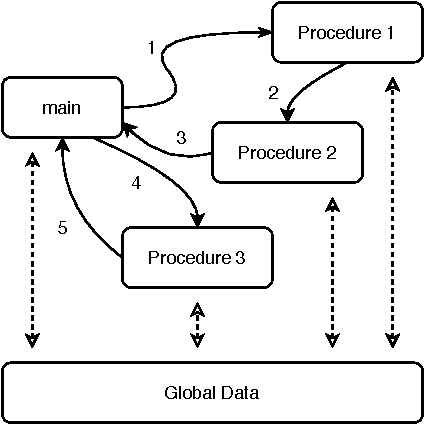
\includegraphics[width=0.50\textwidth]{images/01_2_procedural_programming.pdf}
    \caption{Programmazione procedurale}
    \label{fig:procedural-programming}
\end{figure}
Quando una procedura ha terminato il suo compito il controllo ritorna nuovamente al main (o alla procedura che ne ha effettuato l’invocazione) che esegue una nuova chiamata ad un’altra procedura fino alla terminazione del programma.

\subsubsection{Programmazione modulare}
Questo paradigma rapprenta un ulteriore passo avanti rispetto ai precedenti. La programmazione modulare risponde all'esigenza di poter \textit{riutilizzare le procedure messe a disposizione da un programma in modo che anche altri programmi ne possano trarre vantaggio}. L’idea alla base di questo paradigma è quella di raggruppare le procedure aventi un dominio comune (ad esempio, procedure che eseguono operazioni matematiche) in moduli separati. Quando si parla di \textbf{librerie di programmi}, in sostanza si fa riferimento proprio a moduli di codice indipendenti che ben si prestano ad essere riutilizzati in svariati programmi.
\begin{figure}[H]
    \centering
    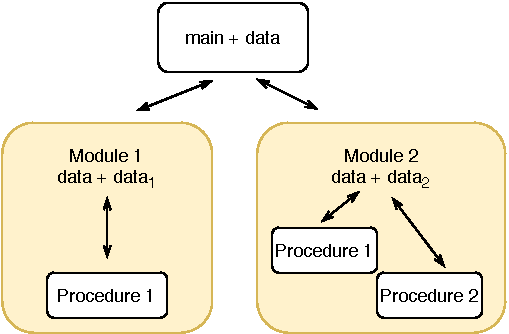
\includegraphics[width=0.50\textwidth]{images/01_3_modular_programming.pdf}
    \caption{Programmazione modulare}
    \label{fig:modular-programming}
\end{figure}
Con questo paradigma un singolo programma non è più costituito da un solo file (in cui è presente il main e tutte le procedure) ma da diversi moduli. Un singolo modulo può contenere anche dei dati propri che, in congiunzione ai dati del main, vengono utilizzati all’interno delle procedure in essi contenuti.

\subsection{Definizione}
\textit{Cosa si intende quindi quando si parla di programmazione a oggetti?} Con il termine programmazione orientata agli oggetti (da qui in seguito \textit{OOP}, in riferimento all'acronimo inglese) si pensa a un insieme di dati come a un singolo oggetto. Più oggetti possono interagire vicendevolmente, scambiandosi messaggi ma mantenendo ciascuno il proprio stato e i propri dati. Questa \textit{rivoluzione del metodo di programmazione} cambia l'approccio mentale all'analisi progettuale, ma non rinuncia ai vantaggi fino ad ora introdotti dai paradigmi precedenti, in particolare a quelli derivanti dall'utilizzo dei moduli. L’idea alla base di questo principio risiede, in buona parte, nel mondo reale. Un \textit{oggetto} è tipicamente un oggetto del mondo reale. In questo paradigma non ha importanza l'implementazione del codice ma, piuttosto, \textbf{le caratteristiche e le azioni} che un componente software è in grado di svolgere e che mette a disposizione di altri oggetti.  
\begin{figure}[H]
    \centering
    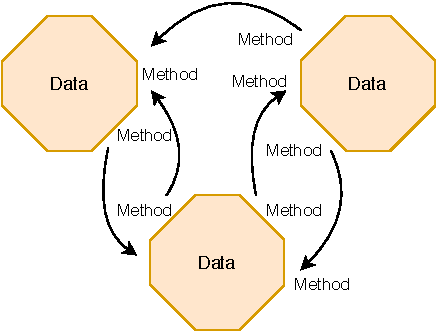
\includegraphics[width=0.50\textwidth]{images/01_4_object_oriented_programming.pdf}
    \caption{Colloquio tra oggetti}
    \label{fig:objectoriented-programming}
\end{figure}
Nella figura gli oggetti sono rappresentati dagli esagoni, che contengono i dati e comunicano attraverso metodi. Nella OOP, i dati (o caratteristiche dell'oggetto), prendono il nome di \textbf{proprietà}, mentre le azioni che essi possono fare \textbf{metodi}. Le proprietà vengono utilizzate dai metodi per eseguire determinate operazioni. Con l'espressione \textbf{pensare “ad oggetti”} quindi si identificano gli oggetti che entrano in gioco nel programma che si vuole sviluppare, gestendone l’interazione degli uni con gli altri.

\subsection{Java | Oracle}
\setlength{\epigraphwidth}{.6\textwidth}
\epigraph{<<The fact that you know Java doesn’t mean that you have the ability to transform that knowledge into well-designed object oriented systems>>}{Paul R. Reed}.\cite{reed:developingapplications}

La nascita del linguaggio Java alla fine del XX secolo segnò un punto di svolta per la programmazione a oggetti. La prima grande rivoluzione introdotta da questo linguaggio fu quella di liberare il programmatore dall'onere della gestione della memoria, che prima era gestita mediante l'utilizzo dei puntatori. Grazie a un sistema chiamato \textbf{garbage collector}, Java è in grado di assegnare e rilasciare automaticamente la memoria in base alla gestione del programma. La seconda rivoluzione introdotta è legata alla Java Virtual Machine (JVM), grazie alla quale i programmi non sono più compilati in codice macchina, ma in una sorta di linguaggio macchina “intermedio” (chiamato bytecode) che non è destinato ad essere eseguito direttamente dall’hardware ma che deve essere, a sua volta, interpretato da un secondo programma, la macchina virtuale appunto. In questo modo lo stesso codice può essere eseguito su più piattaforme semplicemente trasferendo il bytecode (non il sorgente) purché sia disponibile una JVM. Questo concetto prende il nome di \textbf{WORA}, \textit{write once, run everywhere}. Java fu incorporato da diversi web browser per permettere l'utilizzo delle \textit{applet}, un'applicazione che può essere avviata dall'utente eseguendo il codice scaricato da un server web remoto. 

\paragraph*{Perché Java?} Il linguaggio di programmazione è stata la prima decisione per un'ottimale azione di refactoring dell'applicazione e Java si è dimostrato essere il migliore per l'obiettivo dell'elaborato. Il rifacimento del backend è il primo passo sulla strada che porterà Zerocoda a un'evoluzione con conseguente inserimento in un panorama più ampio. Per questo motivo, la quasi totale indipendenza di Java dalla piattaforma hardware di esecuzione è una necessità chiave per l'applicazione, che così acquisisce una maggiore scalabilità. 

\subsubsection{La popolarità}
Prendendo in analisi i grafici offerti da \emph{TIOBE Programming Community Index} \cite{jansen:tiobe}, Java sembrerebbe essere al primo posto. Si tratta di un linguaggio facilmente manutenibile e dotato di molta documentazione che ne facilita l'apprendimento. Con le diverse librerie e framework compatibili è diventato il linguaggio di programmazione a oggetti più utilizzato al mondo, primo anche al precursore C++, dove la gestione della memoria e la curva di apprendimento possono rappresentare un problema. Java è stato adottato per la realizzazione del backend di diversi siti web di rilievo, come il sito d'asta e vendita online \textit{Ebay.com}.

\subsubsection{Le motivazioni}
Uno dei più grandi vantaggi offerti da questo linguaggio è proprio la sua capacità di addattamento ad aggiornamenti e modifiche del software in corso d'opera. Per capire meglio il perchè di questa scelta, facciamo riferimento al seguente esempio:
\begin{figure}[H]
    \centering
    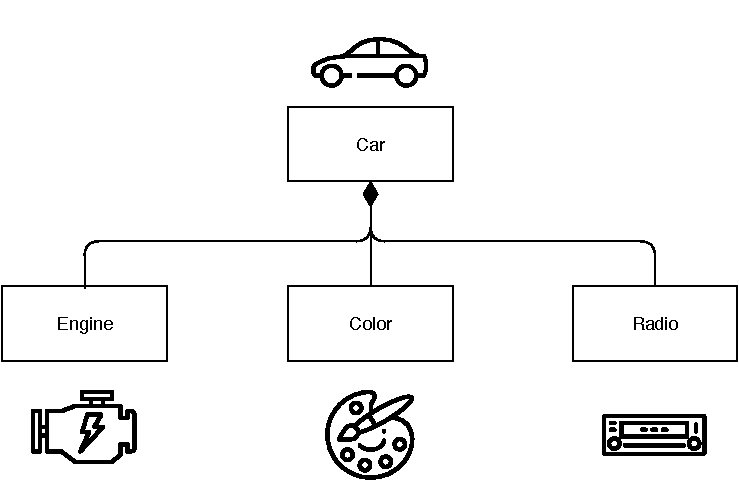
\includegraphics[width=0.75\textwidth]{images/01_5_java_class_diagram.pdf}
\end{figure}
Si pensi ad un rivenditore di auto che ha vari veicoli nel suo parco mezzi. Ogni veicolo è un \texttt{oggetto}, ma ognuno ha caratteristiche diverse denominate \texttt{classi}, che nel nostro esempio sono i diversi modelli, motori, colori della carrozzeria\dots Un cliente sceglie una macchina rossa, ma desidera aggiungere un impianto stereo migliore. La nuova macchina erediterà tutte le caratteristiche dell'oggetto "car" lasciando al programmatore il compito semplificato di modificare solamente la classe “radio” piuttosto che costruire da capo l’intero veicolo. Questo è ciò che rende Java la piattaforma ideale per i telefoni cellulari, i siti web, le console di gioco e qualsiasi applicazione che richieda aggiornamenti e modifiche frequenti.

%%%%%%%%%%%%%%%%%%%%%%%%%%%%%%%%%%%%%%%%%%%%%%%%%%%%%%%%%%%%%%%%%%%%%%%%%
\section{Database Relazionali}
Nello svolgimeto di ogni attività, sia a livello individuale sia in organizazioni di ogni dimmensione, sono essenziali la disponibilità di informazioni e la capacità di gestirle in modo efficiente. \cite{book:basididati} Un database relazionale è un tipo di database di archiviazione che fornisce accesso a data points tra i quali sussistono relazioni predefinite e che soddisfa queste esigenze. I database relazionali sono basati sul modello relazionale, un modello di rappresentazione dati semplice e diretto basato sull'utilizzo di tabelle.

\subsection{Modello Relazionale}
Il modello relazionale si basa su due concetti: \textbf{relazione} e \textbf{tabella}. La nozione di \textit{relazione} proviene dalla matematica, in particolare dalla teoria degli insiemi, mentre il concetto di \textit{tabella} è intuitivo. Il punto di forza del modello di database relazionale è l'uso delle tabelle, che permettono di archiviare informazioni strutturate e accedervi, risultando comprensibili anche per gli utenti finali.
\begin{table}[H]
    \centering
    \begin{tabular}{ |p{2cm}||p{2cm}|p{2cm}|p{3cm}|  }
        \hline
        Matricola & Cognome & Nome & Data di nascita\\
        \hline
        276545 & Rossi & Maria & 25/11/1996\\
        485745 & Neri & Fabio & 23/04/1997\\
        \hline
    \end{tabular}
\end{table}
\begin{table}[H]
    \centering
    \begin{tabular}{ |p{2cm}||p{2cm}|p{2cm}|  }
        \hline
        Studente & Corso & Voto\\
        \hline
        276545 & Analisi & 28\\
        485745 & Chimica & 27\\
        \hline
    \end{tabular}
\end{table}
\begin{itemize}
    \item l'ordine delle colonne e delle righe all'interno di una tabella è insignificante
    \item non possono esistere due righe identiche, ogni riga può essere contrassegnata con un identificatore univoco (chiave principale) che ne faciliti la distinzione dalle altre
    \item  ogni colonna in una tabella ha un nome univoco e contiene un solo tipo di dato
    \item un campo (o cella) può contenere un solo valore effettivo di un attributo
    \item le righe di tabelle diverse possono essere correlate utilizzando chiavi esterne
\end{itemize}

\subsection{Struttura}
Secondo il modello relazionale, le strutture dei dati logici, ovvero tabelle di dati, viste e indici, sono separate dalle strutture di storage fisiche. Grazie a questa separazione, gli amministratori di database possono gestire lo storage fisico dei dati senza compromettere l'accesso a tali dati come struttura logica. Questo permette di accedere ai dati in modi diversi senza riorganizzare le tabelle e di ottenere quindi \textbf{l'indipendenza fisica dei dati}.

\subsection{Database non Relazionali}
Questo tipo di struttura dati si differenzia da quella appena presentata dal momento che non richiede uno schema fisso. La base su cui poggia tutta la costruzione dei database di questo tipo non è costituita da tabelle di dati ma da documenti. La forza di questo principio è proprio che tutto quello che serve all’applicazione risiede nel documento già precompilato. Si evita le frammentazione dell’informazione e la sua ricostruzione, con i rischi di perdere dati o averne di corrotti. Un aumento di flessibilità che velocizza le operazioni e offre risposte più veloci all'utente finale.
\begin{figure}[H]
    \centering
    \begin{minted}{JSON}
        {
            "276545" : {
                "cognome" : "Rossi",
                "nome" : "Maria",
                "data_di_nascita" : "25/11/1996",
                "esami" : [
                    {
                        "corso" : "Analisi",
                        "voto" : 28,
                    }
                ]
            },
            "485745" : {
                "cognome" : "Neri",
                "nome" : "Fabio",
                "data_di_nascita" : "23/04/1997",
                "esami" : [
                    {
                        "corso" : "Chimica",
                        "voto" : 27,
                    }
                ]
            },
        }
    \end{minted}
    \caption{Esempio di documento di un database non relazionale}
    \label{fig:nonrelational-database}
\end{figure}

\subsection{Le differenze}
Un database non relazionale (chiamato anche \textit{NoSQL}) è preferibile quando si ha a che fare con una grande quantità di dati. Questa sua struttura, molto aperta ad aggiunte e scalabile orizzontalmente, rappresenta una grande fattore di rischio per un problema che nei database relazionali è gestito in maniera ottimale: la duplicazione dei dati. Un aspetto che tuttavia depone a favore dei database non relazionali lo si trova nell'\textbf{inserimento dei dati}. Se da una parte per i database NoSQL l'inserimento dei dati risulta più facile e privo di rischi, per i database relazionali un cattivo inserimento può portare alla corruzione dei legami tra tabelle, e quindi all'ottenimento di dati poco edificabili. 

\subsubsection{Integrità dei dati} 
Con un database NoSQL è possibile costruire un documento adatto alla mappatura delle classi-oggetto del proprio applicativo riducendo di molto i tempi di sviluppo. La \textit{mancanza dei controlli fondamentali sull'integrità dei dati}, tuttavia, delega all'applicativo che dialoga con il database questo compito, che ovviamente dovrà essere testato in maniera più approfondita prima di essere messo in produzione. Nei database relazionali questo tipo di controllo avviene all'interno dello stesso database. 

\subsection{MySQL}
Quotidianamente, immense quantità di informazioni vengono affidate a tecnologie che ne garantiscono la conservazione duratura ed un recupero efficiente che ne permetta l’analisi. Da anni, questo ruolo viene interpretato molto bene da un prodotto software completo, efficiente ed affidabile: MySQL. Questo software è un DBMS (database management system) open source per la gestione di database relazionali e rappresenta una delle tecnologie più note e diffuse nel mondo dell'IT. I programmi che dovranno interagire quindi con una base di dati non potranno farlo direttamente, ma dovranno dialogare con il DBMS, che sarà l’unico ad accedere fisicamente alle informazioni.
\begin{figure}[H]
    \centering
    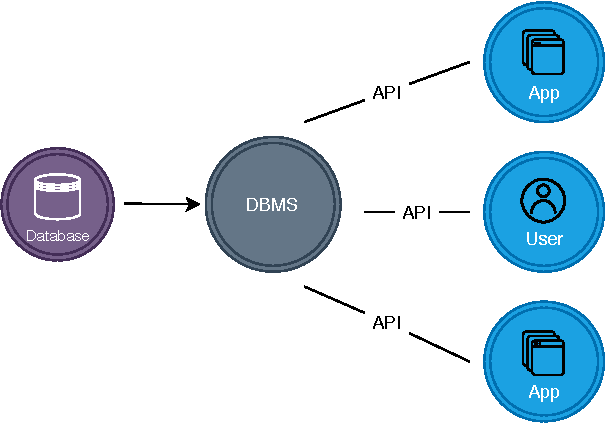
\includegraphics[width=0.65\textwidth]{images/01_6_dbms.pdf}
    \caption{Database management system}
    \label{fig:databasemanagementsystem}
\end{figure}
Oltre alla gestione del database, un DBMS deve controllarne l'accesso concorrente, assicurarne la sicurezza e l'integrità dei dati e permetterne la condivisione e l'integrazioni con applicazioni differenti. Grazie a queste caratteristiche le applicazioni che vengono sviluppate possono contare su una sorgente dati sicura, affidabile e generalmente scalabile.

\subsubsection{Il linguaggio SQL}
Il nome SQL deriva l’abbreviazione di \textit{Structured Query Language}, un linguaggio di programmazione che consente di accedere e gestire i dati in un database relazionale. Questo linguaggio rappresenta lo \textbf{standard per database basati sul modello relazionale}. La diffusione di SQL è dovuta in buona parte alla intensa opera di standardizzazione dedicata a questo linguaggio, svolta principalmente nell'ambito degli organismi ANSI (\textit{American national Standards Institute}, l'organismo nazionale statunitense degli standard) e ISO (l'organismo internazionale che coordina i vari organismi nazionali).

\paragraph{Funzionalità e Sintassi} A seconda dell'operazione che si vuole eseguire sul database, SQL mette a disposizione diverse tipologie di linguaggi:
\begin{itemize}
    \item \textit{DDL - Data Definition Language} per creare e modificare \texttt{schemi di database}
    \item \textit{DML - Data Manipulation Language} inserire, modificare e gestire dati memorizzati
    \item \textit{DQL - Data Query Language} per interrogare i \texttt{dati memorizzati}
    \item \textit{DCL - Data Control Language} creare e gestire strumenti di controllo e accesso ai dati
\end{itemize}
Sarebbe quindi diminutivo definire SQL 'un semplice linguaggio di interrogazione' in quanto alcuni dei suoi sottoinsiemi sopra elencati permettono di creare, gestire e modificare il database. La popolarità di SQL è inoltre dovuta alla sua facilità di comprensione, dovuta a un linguaggio con comandi semplici, autoesplicativi nella loro sintassi, e prestante per qualsiasi tipo di operazione.
\begin{figure}[H]
    \centering
    \begin{minted}{SQL}
        SELECT Matricola, Cognome, Nome, Corso, Voto 
        FROM Studenti JOIN Esami 
        ON Matricola = Studente
    \end{minted}
    \caption{Esempio di query SQL}
    \label{fig:sql-example}
\end{figure}
\begin{table}[H]
    \centering
    \begin{tabular}{ |p{2cm}||p{2cm}|p{2cm}|p{2cm}|p{2cm}|  }
        \hline
        Matricola & Cognome & Nome & Corso & Voto\\
        \hline
        276545 & Rossi & Maria & Analisi & 28\\
        485745 & Neri & Fabio & Chimica & 27\\
        \hline
    \end{tabular}
\end{table}

%%%%%%%%%%%%%%%%%%%%%%%%%%%%%%%%%%%%%%%%%%%%%%%%%%%%%%%%%%%%%%%%%%%%%%%%%

\section{Architettura di Microservizi}
\subsection{Architettura Monolitica}
Ai primordi dello sviluppo applicativo, anche un cambiamento minimo  a un software esistente imponeva un aggiornamento completo e un ciclo di controllo qualità. Le applicazioni erano sviluppate e distribuite come una singola entità, e tale approccio veniva spesso definito \textbf{“monolitico”}, perché il codice sorgente dell’intera applicazione era compilato in una singola unità di deployment. 

\begin{figure}[H]
    \centering
    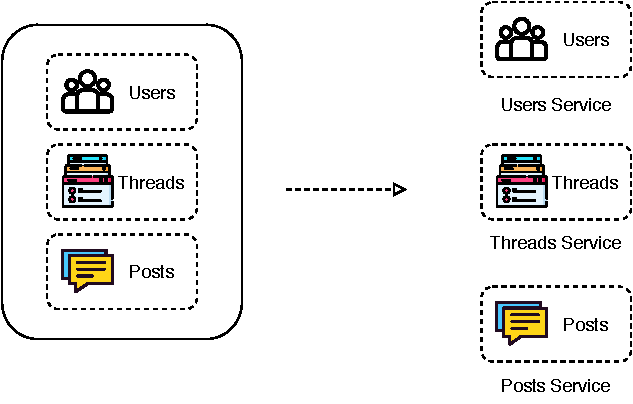
\includegraphics[width=0.75\textwidth]{images/01_7_monolithic_vs_microservices.pdf}
    \caption{Architettura Monolitica e Microservizi }
    \label{fig:monolithicvsmicroservices}
\end{figure}

\paragraph{Caratteristiche} Le applicazioni che seguono questo tipo di architettura sono di facile implementazione, in quanto tipicamente raccolte all'interno di un unico progetto e distribuite in un unico pacchetto. Questo tipo di architettura si presta bene per applicazioni piccole o comunque poco soggette a cambiamenti, ma la cosa cambia quando ci troviamo a sviluppare applicazioni complesse che richiedono continui aggiornamenti. Se uno di questi dovesse causare errori, l'unica soluzione sarebbe quella di \textit{disconnettere tutto} e fare un rollback totale del software: è chiaro che un'azienda non può permettersi tempi di inattività. L’unico modo di poter scalare un’applicazione monolitica è quello di replicare l’intera applicazione con conseguente aumento di costi e risorse necessarie. In seguito ai problemi derivanti da questo tipo di architettura, nacquero i primi studi di archittetture a servizi, sulla base di uno dei dogmi dell'ingegneria del software:

\newtheorem{defin}{Principio di Singola Responsabilità}
\begin{defin}
    Riunire le cose che cambiano per lo stesso motivo e separare quelle che cambiano per motivi diversi.
\end{defin}

\subsubsection{Cosa sono i Microservizi}
L'architettura di microservizi rappresenta un'approccio all'avanguardia per lo sviluppo e l'organizzazione del software. Secondo questo stile, il software è composto da servizi indipendenti di piccole dimensioni che hanno come finalità lo svolgimento di un unico compito, e di farlo nel migliore dei modi. \cite{amazon:microservices} Ciascun microservizio, indipendente dagli altri, è dunque gestito da un unico team di sviluppo. Per una definizione più precisa riprendiamo le parole di Martin Fowler, considerato uno dei massimi esperti in materia, che afferma: \textit{<<Lo stile architetturale a microservizi è un approccio allo sviluppo di una singola applicazione come insieme di piccoli servizi, ciascuno dei quali viene eseguito da un proprio processo e comunica con un meccanismo snello, spesso una HTTP API.>>} \cite{fowler:microservices}

\subsection{Le origini}
Il primo tentativo di architettura a servizi nasce con l’\texttt{architettura SOA}. Il concetto delle \textit{Service-Oriented Architecture} si afferma all’inizio degli anni Duemila come una collezione di servizi indipendenti che comunicano gli uni con gli altri tramite un \textit{Enterprise Service Bus (ESB)}. L’architettura a microservizi è una chiara \textbf{evoluzione dell’architettura SOA}, spinta dall’esigenza  di una sempre più’ marcata scalabilità, la quale permette di reggere il carico di milioni di utenti connessi in un determinato istante.

\subsection{Le differenze con SOA}
Per studiare le differenze tra le due architettura facciamo riferimento al seguente schema:
\begin{figure}[H]
    \centering
    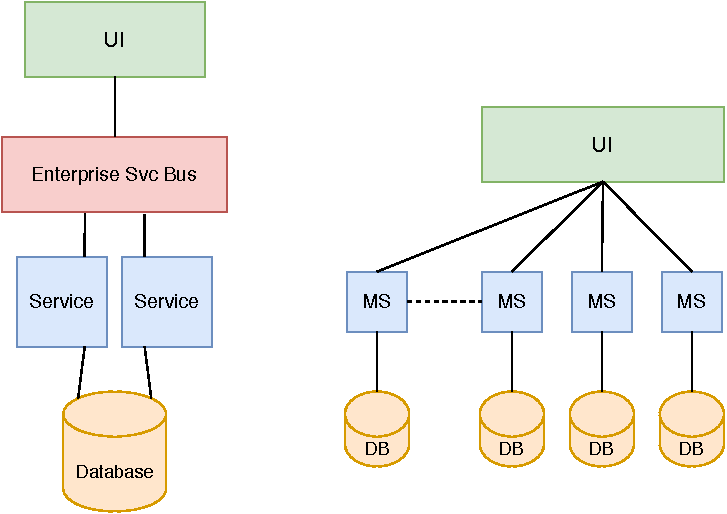
\includegraphics[width=0.80\textwidth]{images/01_8_microservices_vs_soa.pdf}
    \caption{Architettura SOA e Microservizi }
    \label{fig:soavsmicroservices}
\end{figure}
\paragraph*{Granularità dei Servizi} Il numero dei servizi è un buon fattore per la differenziazione delle due architetture. Lo stesso Martin Fowler, citato precedentemente, afferma che in un'architettura SOA non si arriva neanche ad una decina di  servizi mentre in un architettura a microservice il numero dei servizi e’ molto più alto: basti pensare che il servizio di streaming Netflix ha dichiarato di fare uso di oltre di 700 microservizi. \cite{article:netflixmicroservices}

\paragraph{Comunicazione} I microservizi abbandonano l’utilizzo di ESB, comunicando direttamente tra loro con meccanismi di comunicazione light. Nella SOA, l’ESB potrebbe diventare un singolo punto di errore che influisce sull’intero sistema. Poiché ogni servizio comunica attraverso l’ESB, se uno dei servizi rallenta, potrebbe ostruire l’ESB con le richieste per quel servizio. D’altra parte, i microservizi sono molto migliori nella tolleranza agli errori: se un microservizio presenta un errore di memoria, verrà interessato solo quel microservizio.

\paragraph{Database} In SOA i servizi condividono gli storage mentre con i microservice ogni servizio può avere un database indipendente.

\subsection{Caratteristiche dei Microservizi}

\subsubsection{Autonomia}
Ciascun servizio nell’architettura basata su microservizi può essere sviluppato, distribuito, eseguito e ridimensionato senza influenzare il funzionamento degli altri componenti. I servizi non condividono alcun codice o implementazione con gli altri.

\subsubsection{Specificità}
Ciascun servizio è progettato per una serie di capacità e si concentra sulla risoluzione di un problema specifico. Se nel tempo si decide di rendere un servizio più complesso, il servizio può essere scomposto in servizi più piccoli.

\subsubsection{Eterogeneità delle Tecnologie}
Durante lo sviluppo di un microservizio si ha totale libertà di scelta nell'utilizzo delle tecnologie. Ciascuna tecnologia viene decisa esclusivamente in base allo scopo del microservizio, senza basarsi sulla sua interazione con gli altri. Un microservizio può fare affidamento su un modello di database relazionale mentre un servizio con cui comunica su uno di tipo non relazionale, così come la loro logica può essere scritta in linguaggi differenti.

\subsubsection{Semplicità di Distribuzione}
Con i microservizi è possibile apportare una modifica a un singolo servizio e distribuirlo indipendentemente dal resto del sistema con tecniche di continuos delivery del tutto automizzate. Questo permette di rilasciare aggiornamenti più velocemente e in maniera più sicura.

\subsubsection{Resilienza}
La resilienza è la capacità di accettare la possibilità’ di errori e continuare a funzionare. Con i microservizi, le applicazioni possono gestire completamente gli errori di un servizio isolando la funzionalità senza bloccare l’intera applicazione.

\subsubsection{Scalabilità}
I microservizi consentono di scalare ciascun servizio in modo indipendente per rispondere alla richiesta delle funzionalità che un'applicazione supporta. 

%%%%%%%%%%%%%%%%%%%%%%%%%%%%%%%%%%%%%%%%%%%%%%%%%%%%%%%%%%%%%%%%%%%%%%%%%

\section{Representational State Transfer - REST}
\subsection{Cos'è un'API}
Un'\textit{Application Program Interface} può essere considerata come un \textsc{contratto} tra un fornitore di informazioni e l'utente destinatario di tali dati: l'API si limita a stabilire il contenuto richiesto dal consumatore (la chiamata) e il contenuto richiesto dal produttore (la risposta). Un'API funge quindi da elemento di intermediazione tra gli utenti e le risorse che questi intendono ottenere. È anche un mezzo con il quale un'organizzazione può condividere risorse e informazioni assicurando al contempo sicurezza e controllo, poiché stabilisce i criteri di accesso. L'utilizzo di un'API permette all'utente di rimanere all'oscuro delle specifiche con cui le risorse vengono recuperate o della loro provenienza.
\begin{figure}[H]
    \centering
    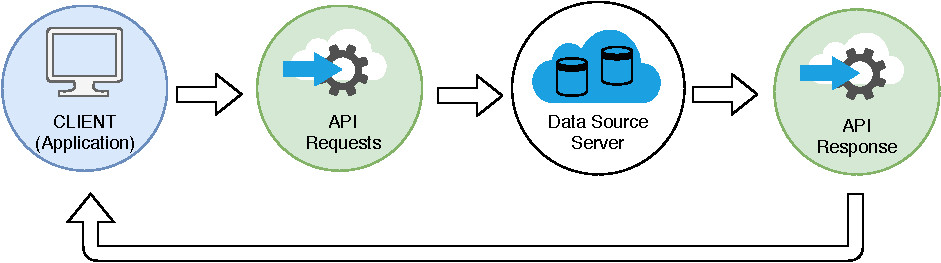
\includegraphics[width=0.90\textwidth]{images/01_9_api.pdf}
    \caption{Funzionamento delle API}
    \label{fig:api}
\end{figure}

\subsection{L'architettura REST}
Il Representational State Transfer è lo stile architetturale più popolare degli ultimi anni. Non si tratta di un protocollo nè tantomeno di una specifica (in quanto non fa riferimento a uno standard ufficiale), ma piuttosto di una serie di vincoli per la creazione di un servizio web che può servirsi di standard,  come HTTP, URI, JSON e XML. REST permette di \textit{accedere} e \textit{modificare} la \textbf{rappresentazione testuale di risorse}, attraverso una serie di \textbf{operazioni stateless} \textit{uniformi} e \textit{predefinite}. Generalmente basato su HTTP, permette di utilizzare anche altri protocolli di trasferimento come SNMP, SMTP, ecc\dots

\paragraph{Perchè è conveniente?} L'utilizzo di API Rest fornisce una notevole quantità di libertà e flessibilità agli sviluppatori. Questo stile architetturale non richiede l'installazione di alcuna libreria (fatta eccezione per HTTP Client-Server e il JSON parser). Non vincola  chi lo sceglie a utilizzare una tecnologia, ma al contrario ne supporta diverse.

\paragraph{Cosa la rende semplice?} L'informazione, o rappresentazione, viene consegnata in uno dei diversi formati tramite HTTP: JSON (Javascript Object Notation), HTML, XLT o testo semplice. Il formato JSON è uno dei più diffusi, perché indipendente dal linguaggio e facilmente leggibile da persone e macchine.
\begin{figure}[H]
    \centering
    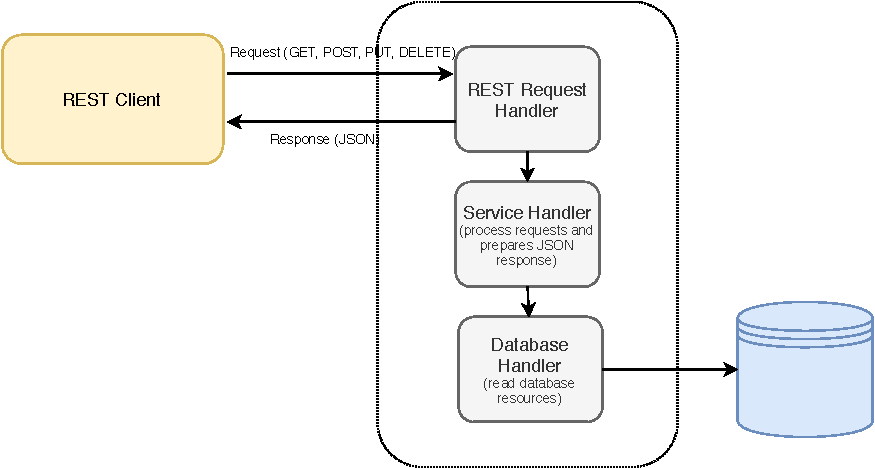
\includegraphics[width=0.95\textwidth]{images/01_10_restapi.pdf}
    \caption{Funzionamento delle API Rest}
    \label{fig:api}
\end{figure}

\subsubsection{Principi REST}
Di seguito esponiamo i \textit{sei principi per un'architettura REST}, per la prima volta introdotti durante la dissertazione nella tesi di dottorato di Roy Fielding, uno dei principali autori delle specifiche dell'Hypertext Transfer Protocol (HTTP). \cite{fielding:restprinciples}

\paragraph{1. Client-Server} Secondo questo principio, nello sviluppo di un'architettura REST Client e Server devono rimanere separati, in modo da potersi evolvere individualmente. Per questo motivo, si dice che rispetta il paradigma dell'informatica noto come \textbf{Separation of Concerns (SoC)}, traducibile in italiano come \emph{suddivisione dei compiti}. Secondo il principio SoC il sistema deve essere diviso in moduli distinti, ciascuno dedito allo svolgimento di un proprio compito, supportando in tal modo l’evoluzione indipendente della logica lato client e della logica lato server. Secondo questo vincolo il server deve offrire una o più funzionalità e ascoltare le richieste di possibili client. Un client deve invocare il servizio messo a disposizione dal server inviando il corrispondente messaggio di richiesta. Il servizio lato server a questo punto respinge la richiesta o esegue l’attività richiesta prima di inviare un messaggio di risposta al client. La gestione delle eccezioni è delegata al client.

\paragraph{2. Stateless} Con questo termine si fa riferimento al tipo di operazioni. Le singole invocazioni delle API Rest non devono fare affidamento alle risorse presenti sul server, ma esclusivamente sui dati forniti nella stessa richiesta. Nel client non è previsto un sistema di memorizzazione delle informazioni delle richieste, ciascuna di queste è distinta e non connessa. Ciò garantisce una forte scalabilità, riducendo l'utilizzo di memoria sul server.

\paragraph{3. Cache} Le Rest API devono essere progettate in modo da favorire l'utilizzo di date cachable. \emph{La richiesta di rete più efficiente è quella che non utilizza la rete.} In un 'architettura REST i messaggi di risposta dal servizio ai suoi consumatori sono esplicitamente etichettati come memorizzabili nella cache oppure non memorizzabili. In questo modo, il servizio, il consumatore o uno dei componenti intermediari possono memorizzare nella cache la risposta per il riutilizzo nelle richieste successive. Le richieste vengono passate attraverso un componente cache, che può riutilizzare le risposte precedenti per eliminare parzialmente o completamente alcune interazioni sulla rete.

\paragraph{4. Interfaccia Uniforme}

\paragraph{5. Sistema a strati}

\paragraph{6. Codice su richiesta}

\subsection{Web Service SOAP}